%
% Example file
%

\documentclass{fose2019}           % for pLaTeX2e
%\documentclass[english]{fose2016} % for English papers
%\documentclass[ascii]{fose2016}   % for ASCII pTeX

\usepackage[dvipdfmx]{graphicx}
%\usepackage{epsfig}
\usepackage{comment}
\usepackage{graphicx}
\usepackage{multirow}
\usepackage{tabularx}



\title{類似コード検出ツールを用いたテストコード再利用に向けた調査}
\etitle{Investigation for test code reuse using similar code detection tool}
\journalhead{An example of use for fose2019.cls}
\author{倉地 亮介}{Ryosuke Kurachi, 奈良先端科学技術大学院大学}
\author{崔 恩瀞}{Eunjong Choi, 京都工芸繊維大学}

\begin{document}

\maketitle


\begin{abstract}
テストコード自動生成ツールによって生成されるテストコードは開発者の保守作業を困難にする課題がある.我々は,解決方法として既存テストの再利用によるテストコード自動生成ツールを提案する.本研究では,提案ツールの実現に向けて類似コードペアの分類を行い,類似コードペア間の類似度とテストコードペア間の類似度の関係を調査した.
\end{abstract}

\begin{comment}
\section{はじめに}
近年,ソフトウェア開発に求められる要件が高度化・多様化する一方で,ユーザからはソフトウェアの品質確保やコスト削減に対する要求も増加している\cite{1}.その中でもソフトウェアのテスト工程は開発全体のコストに占める割合が大きく,品質確保の要である.しかし,現状ではテスト作成作業の大部分が人手で行われており,多くのテストを作成しようとするとそれに比例してコストも増加してしまう.このような状況の中で,ソフトウェアの品質を確保しつつコスト削減を達成するために単体テストのテストコード自動生成ツールの利用が進んでいる.しかし,既存の自動生成ツールによって自動生成されたテストコードは,対象コードの作成経緯や意図に基づいていないという性質から開発者の保守作業を困難にする課題がある[2].我々は,この課題の解決方法として既存テストの再利用によるテストコード自動生成ツールが必要であると考える.既存テストを再利用する方法として,類似コード間でのテスト再利用手法を提案する.この手法は,テストコードがないコード片aに対して,類似したコード片a'を検索し,その類似コード片に対応するテストコードをコード片aに再利用する方法である.一般に,ソースコードの再利用は生産性や信頼性,コスト等の改善につながると言われている.一方でソースコードの再利用は,対象となるソースコードを十分に理解し利用する必要があるため非常に困難なタスクであると考えられている[3].これは,テストコードの再利用についても同様に難しいと考えられる.そのため,どのようなテストコードが類似コード間で再利用できるのかを明らかにすることがテストコードの再利用支援において重要である.本研究では,既存のJavaプロジェクト内の類似コードペアをテストコードの有無によって分類し,プロジェクト内に存在する再利用候補となる類似コードペアの割合と,類似コードペアの類似度とテストコードの類似度の関係を調査した.その結果,類似コードペアとテストコードの類似度には相関があることが分かった.
\end{comment}

\section{はじめに}
ソフトウェア開発のテスト工程において,テスト作成コストを削減するためにテストコード自動生成ツールの利用が進んでいる.しかし,既存のツールによって生成されるテストコードはテスト対象コードの作成経緯や意図に基づいていないという性質から開発者の保守作業を困難にする課題がある\cite{1}.そこで,解決方法として既存テストの再利用によるテストコード自動生成ツールが必要であると考える.
\\\indent 我々は,テストの再利用手法として,類似コード間でのテスト再利用手法を提案する.この手法は,類似コード検出ツール\cite{Nicad}を用いてテストコードがないコード片aに対して類似したコード片a'を検出し,その類似コード片に対応するテストコードをコード片aに再利用する方法である.本手法で,テスト再利用の候補となるのは「どちらか片方のコード片にテストコードが存在する類似コードペア」である.
\\\indent 既存テストの再利用は命名規則に従った保守性の高いテストコードを利用できる.一方で,類似コード間でのテスト再利用は再利用候補となる類似コードペアが存在しないとできないことや,テスト対象となる類似コードペア間の関係に依存するので困難な作業である.そのため,どのようなテストコードが類似コード間で再利用できるのかを明らかにすることがテストコードの再利用支援において重要である.
\\\indent 本研究では,既存のJavaプロジェクト内の類似コードペアをテストコードの有無によって分類し,プロジェクト内に存在する再利用候補となる類似コードペアの割合と,「両方のコード片にテストコードが存在する類似コードペア」を対象に類似コードペア間の類似度とテストコードペア間の類似度の関係を調査した.
\begin{comment}
その結果,類似コードペアの類似度とテストコードの類似度には相関があることが分かった.
\end{comment}

\section{類似コードペアの分類}
調査を行うために,類似コードペアをテストコードの有無によって3種類に分類する.類似コードペアの分類手法は,主に以下の5つのステップから構成される.
\begin{description}
\item[Step1:]プロジェクト内のテストコードとテスト対象コードを収集
\item[Step2:]Step1で得られたテスト対象コードから類似コードペアの検出
\item[Step3:]Step1,2で得られた類似コード片とテストコードをメソッド単位で対応付け
\item[Step4:]Step3の対応付け表からテストコードの有無により類似コードペアを分類
\end{description}

\begin{comment}
\begin{figure}[htbp]
  \centering
  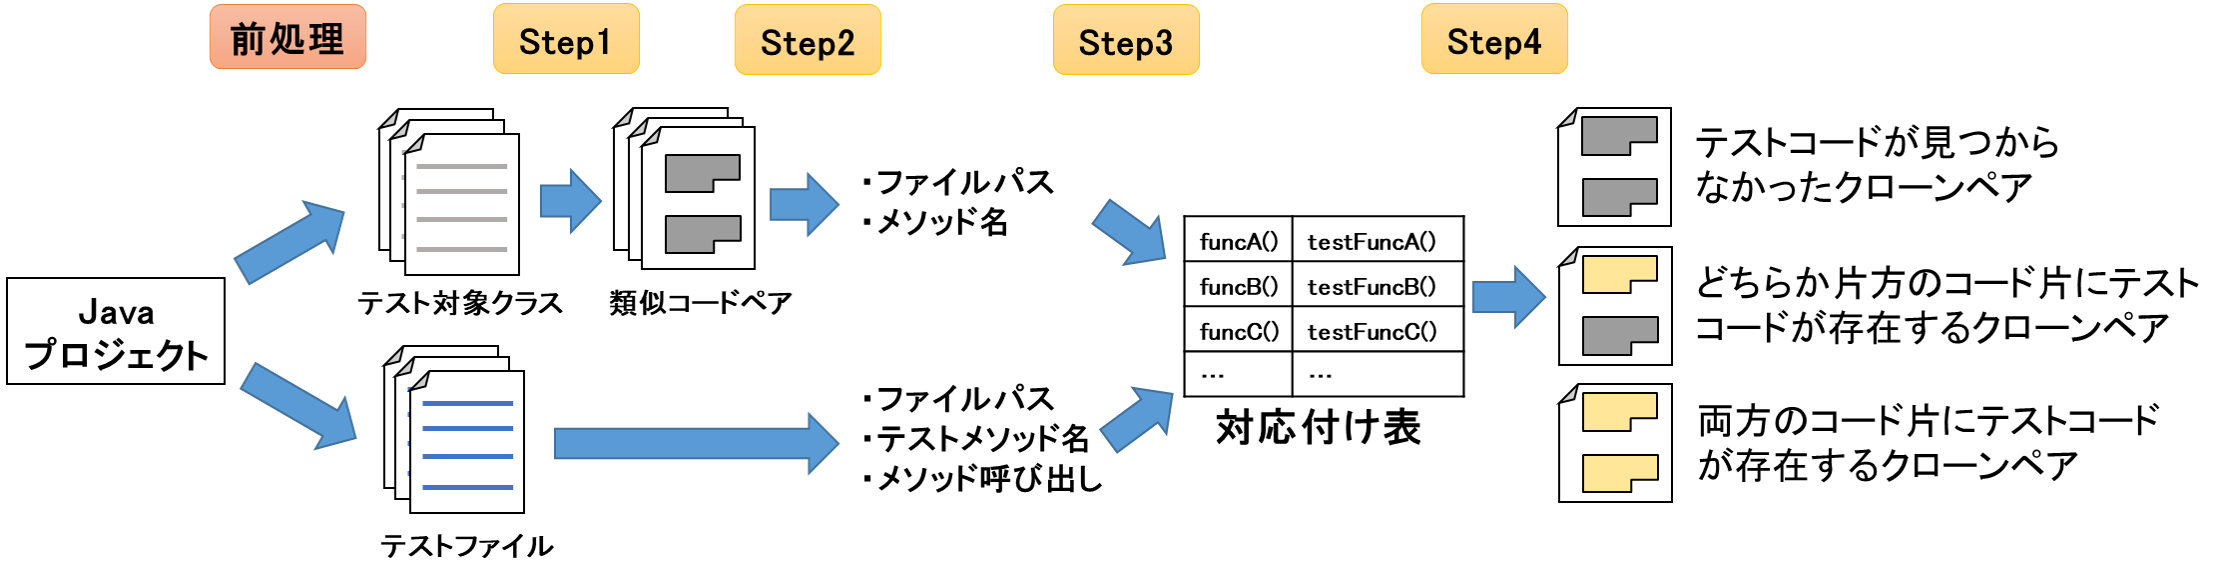
\includegraphics[width=\textwidth]{2.png}
%  
\epsfig{file=fose2005logo.eps,width=\textwidth}
  \caption{類似コードペアの分類手法の概要}
  \label{fig:example}
\end{figure}
\end{comment}
\section{調査概要}
%\begin{comment}
\begin{description}
\item[調査1:]プロジェクト内にテストの再利用候補となる類似コードのペアはどの程度存在するか
%OSSに存在する人気javaプロジェクトを対象に調査を実施し,類似コード間のテスト再利用手法がどの程度有効なのかを明らかにする
\item[調査2:]類似コードペア間の類似度と対応するテストコードペア間の類似度にはどのような関係があるか
%テストコード間の類似度が高いほど再利用できる可能性も高くなると考えられるので,
%「両方のコード片にテストコードが存在する類似コードペア」を対象に類似コードペアの類似度とテストコードの類似度をソースコードの差異の度合いを示すタイプ別に分類し関係性を調査
\end{description}
%\end{comment}

\section{調査結果}
\begin{table}[]
\centering
\caption{既存Javaプロジェクト中の類似コードペアの分類結果}
\begin{tabular}{|c|p{2.5em}|c|p{4em}|c|p{3.5em}|c|c|c|}
\hline
                          & \multicolumn{2}{c|}{\begin{tabular}[c]{@{}c@{}}\scriptsize テストコードが存在\\ \scriptsize しない類似コードペア\end{tabular}} & \multicolumn{2}{c|}{\begin{tabular}[c]{@{}c@{}}\scriptsize どちらか片方のコード片にテスト\\ \scriptsize コードが存在する類似コードペア\end{tabular}} & \multicolumn{2}{c|}{\begin{tabular}[c]{@{}c@{}}\scriptsize 両方のコード片にテストコード\\ \scriptsize が存在する類似コードペア\end{tabular}} & \multicolumn{2}{c|}{\scriptsize 合計}                       \\ \cline{2-9} 
\multirow{-3}{*}{\scriptsize プロジェクト名} & \scriptsize \hfil 数 \hfil                                        & \scriptsize 割合                                       & \scriptsize \hfil 数 \hfil                                             & \scriptsize 割合                                             & \scriptsize \hfil 数 \hfil                                           & \scriptsize 割合                                           & \multicolumn{2}{c|}{\scriptsize 数}  \\ \hline
{\scriptsize Apache maven}             &{\scriptsize \hfil 260 \hfil}                &{\scriptsize 63.9}                & {\scriptsize \hfil 139 \hfil}                      & {\scriptsize 34.2}                     & {\scriptsize \hfil 8 \hfil}                      & {\scriptsize 2.0}                    & \multicolumn{2}{c|}{\scriptsize 407}  \\ \hline
{\scriptsize Apache kafka}             & {\scriptsize \hfil 442 \hfil}                & {\scriptsize 70.8}                & {\scriptsize \hfil 135 \hfil}                      & {\scriptsize 21.6}                    & {\scriptsize \hfil 47 \hfil}                     & {\scriptsize 7.5}                    & \multicolumn{2}{c|}{\scriptsize 624}  \\ \hline
{\scriptsize Apache kylin}             & {\scriptsize \hfil 177 \hfil}                & {\scriptsize 72.2}                &{\scriptsize \hfil 60 \hfil}                       & {\scriptsize 24.5}                     & {\scriptsize \hfil 7 \hfil}                      & {\scriptsize 2.9}                    & \multicolumn{2}{c|}{\scriptsize 245}  \\ \hline
{\scriptsize 合計}                      & {\scriptsize \hfil 879 \hfil}                & {\scriptsize 68.9}                & {\scriptsize \hfil 334 \hfil}                      & {\scriptsize 26.2}                     & {\scriptsize \hfil 62 \hfil}                     & {\scriptsize 4.9}                    & \multicolumn{2}{c|}{\scriptsize 1275} \\ \hline
\end{tabular}
\end{table}

\begin{comment}
\begin{table}[]
\centering
\caption{既存Javaプロジェクト中の類似コードペアの分類結果}
\begin{tabular}{|l|c|c|c|c|}
\hline
    & \multicolumn{4}{c|}{\scriptsize テストコードペアの類似度}         \\ \hline
\scriptsize 類似  &             & \scriptsize Not Similar & \scriptsize type2 &\scriptsize type3 \\ \cline{2-5} 
\scriptsize コード & \scriptsize Not Similar & \scriptsize 21          & \scriptsize 0     & \scriptsize 0     \\ \cline{2-5} 
\scriptsize ペアの & \scriptsize type2       & \scriptsize 6           & \scriptsize 77    & \scriptsize 10    \\ \cline{2-5} 
\scriptsize 類似度 & \scriptsize type3       & \scriptsize 6           & \scriptsize 28    & \scriptsize 5     \\ \hline
\end{tabular}
\end{table}
\end{comment}

\begin{table}[]
\centering
\caption{類似コードペア間の類似度とテストコードペア間の類似度の関係}
\begin{tabular}{|c|c|c|c|c|}
\hline
                             & \multicolumn{4}{c|}{\scriptsize テストコードペア間の類似度}         \\ \hline
\multirow{4}{*}{\scriptsize 類似コードペア間の類似度} &             & \scriptsize Not Similar & \scriptsize type2 & \scriptsize type3 \\ \cline{2-5} 
                             & \scriptsize Not Similar & \scriptsize 21          & \scriptsize 0     & \scriptsize 0     \\ \cline{2-5} 
                             &\scriptsize type2       & \scriptsize 6           & \scriptsize 77    & \scriptsize 10    \\ \cline{2-5} 
                             & \scriptsize type3       & \scriptsize 6           & \scriptsize 28    & \scriptsize 5     \\ \hline
\end{tabular}
\end{table}

\begin{comment}
\begin{minipage}{0.3\hsize}
\begin{tabular}{|c|c|c|p{2.3em}|c|p{1.8em}|c|c|l|}
\hline
                          & \multicolumn{2}{l|}{\begin{tabular}[c]{@{}l@{}}\tiny テストコード\\ \tiny が存在しない\\ \tiny 類似コードペア\end{tabular}} & \multicolumn{2}{l|}{\begin{tabular}[c]{@{}l@{}}\tiny どちらか片方のコード片\\ \tiny にテストコードが存在\\ \tiny する類似コードペア\end{tabular}} & \multicolumn{2}{l|}{\begin{tabular}[c]{@{}l@{}}\tiny 両方のコード片に\\ \tiny テストコードが存在\\ \tiny する類似コードペア\end{tabular}} & \multicolumn{2}{c|}{\scriptsize 合計}                       \\ \cline{2-9} 
\multirow{-2}{*}{\scriptsize プロジェクト名} & \scriptsize \hfil 数 \hfil                                          & \scriptsize 割合                                         & \scriptsize \hfil 数 \hfil                                                & \scriptsize 割合                                              & \scriptsize \hfil 数 \hfil                                              & \scriptsize 割合                                            & \multicolumn{2}{c|}{{\scriptsize 数}} \\ \hline
{\scriptsize Apache maven}             &{\scriptsize \hfil 260 \hfil}                &{\scriptsize 63.9}                & {\scriptsize \hfil 139 \hfil}                      & {\scriptsize 34.2}                     & {\scriptsize \hfil 8 \hfil}                      & {\scriptsize 2.0}                    & \multicolumn{2}{c|}{\scriptsize 407}  \\ \hline
{\scriptsize Apache kafka}             & {\scriptsize \hfil 442 \hfil}                & {\scriptsize 70.8}                & {\scriptsize \hfil 135 \hfil}                      & {\scriptsize 21.6}                    & {\scriptsize \hfil 47 \hfil}                     & {\scriptsize 7.5}                    & \multicolumn{2}{c|}{\scriptsize 624}  \\ \hline
{\scriptsize Apache kylin}             & {\scriptsize \hfil 177 \hfil}                & {\scriptsize 72.2}                &{\scriptsize \hfil 60 \hfil}                       & {\scriptsize 24.5}                     & {\scriptsize \hfil 7 \hfil}                      & {\scriptsize 2.9}                    & \multicolumn{2}{c|}{\scriptsize 245}  \\ \hline
{\scriptsize 合計}                      & {\scriptsize \hfil 879 \hfil}                & {\scriptsize 68.9}                & {\scriptsize \hfil 334 \hfil}                      & {\scriptsize 26.2}                     & {\scriptsize \hfil 62 \hfil}                     & {\scriptsize 4.9}                    & \multicolumn{2}{c|}{\scriptsize 1275} \\ \hline
\end{tabular}
\end{minipage}


\begin{tabular}{|c|c|c|p{2.3em}|c|p{1.8em}|c|c|l|}
\hline
                          & \multicolumn{2}{l|}{\begin{tabular}[c]{@{}l@{}}\tiny テストコード\\ \tiny が存在しない\\ \tiny 類似コードペア\end{tabular}} & \multicolumn{2}{l|}{\begin{tabular}[c]{@{}l@{}}\tiny どちらか片方のコード片\\ \tiny にテストコードが存在\\ \tiny する類似コードペア\end{tabular}} & \multicolumn{2}{l|}{\begin{tabular}[c]{@{}l@{}}\tiny 両方のコード片に\\ \tiny テストコードが存在\\ \tiny する類似コードペア\end{tabular}} & \multicolumn{2}{c|}{\scriptsize 合計}                       \\ \cline{2-9} 
\multirow{-2}{*}{\tiny プロジェクト名} & \tiny \hfil 数 \hfil                                          & \tiny 割合                                         & \tiny \hfil 数 \hfil                                                & \tiny 割合                                              & \tiny \hfil 数 \hfil                                              & \scriptsize 割合                                            & \multicolumn{2}{c|}{{\scriptsize 数}} \\ \hline
{\scriptsize Apache maven}             &{\scriptsize \hfil 260 \hfil}                &{\scriptsize 63.9}                & {\scriptsize \hfil 139 \hfil}                      & {\scriptsize 34.2}                     & {\scriptsize \hfil 8 \hfil}                      & {\scriptsize 2.0}                    & \multicolumn{2}{c|}{\scriptsize 407}  \\ \hline
{\scriptsize Apache kafka}             & {\scriptsize \hfil 442 \hfil}                & {\scriptsize 70.8}                & {\scriptsize \hfil 135 \hfil}                      & {\scriptsize 21.6}                    & {\scriptsize \hfil 47 \hfil}                     & {\scriptsize 7.5}                    & \multicolumn{2}{c|}{\scriptsize 624}  \\ \hline
{\scriptsize Apache kylin}             & {\scriptsize \hfil 177 \hfil}                & {\scriptsize 72.2}                &{\scriptsize \hfil 60 \hfil}                       & {\scriptsize 24.5}                     & {\scriptsize \hfil 7 \hfil}                      & {\scriptsize 2.9}                    & \multicolumn{2}{c|}{\scriptsize 245}  \\ \hline
{\scriptsize 合計}                      & {\scriptsize \hfil 879 \hfil}                & {\scriptsize 68.9}                & {\scriptsize \hfil 334 \hfil}                      & {\scriptsize 26.2}                     & {\scriptsize \hfil 62 \hfil}                     & {\scriptsize 4.9}                    & \multicolumn{2}{c|}{\scriptsize 1275} \\ \hline
\end{tabular}
\end{minipage}

\hfill
\begin{minipage}{0.3\hsize}		
\begin{tabular}{|l|c|c|c|c|}
\hline
    & \multicolumn{4}{c|}{\scriptsize テストコードペアの類似度}         \\ \hline
\scriptsize 類似  &             & \scriptsize Not Similar & \scriptsize type2 &\scriptsize type3 \\ \cline{2-5} 
\scriptsize コード & \scriptsize Not Similar & \scriptsize 21          & \scriptsize 0     & \scriptsize 0     \\ \cline{2-5} 
\scriptsize ペアの & \scriptsize type2       & \scriptsize 6           & \scriptsize 77    & \scriptsize 10    \\ \cline{2-5} 
\scriptsize 類似度 & \scriptsize type3       & \scriptsize 6           & \scriptsize 28    & \scriptsize 4     \\ \hline
\end{tabular}
\end{minipage}
\end{comment}


調査1の結果を表1に示す.3つのJavaプロジェクト中のテスト対象となる類似コードペアの内,26.2\%が再利用候補になることが分かった.この結果は,類似コードペアの中で片方のコード片にはテストコードがあるにも関わらず,もう片方のコード片はテストされていないものが全体の4分の1以上を占めており,提案ツールの実現により多くのコード片にテストコードを再利用できる可能性を示している.
\\\indent 調査2では,類似コードペアの分類によって得られた「両方のコード片にテストコードが存在する類似コードペア」62個とそれに対応するテストコードのペア153個の類似度の関係を表2に示した.調査の結果,テスト対象となる類似コードペアが類似していない(Not Similar)場合は,類似するテストコードペアが存在しないことが分かった.また,類似コードペアの類似度がタイプ2,3の場合は,テストコードの類似度もタイプ2,3が多い結果となった.この結果から,テストコードペアの間の類似度と対象の類似コードペア間の類似度には相関関係があり,類似度が高いほどテストコードを再利用できる可能性を示している.
\\\indent 一方で,類似コードペア間の類似度がタイプ2と高いにもかかわらず,テストコードペアが類似しない組み合わせが6件検出された.これらの類似コードペアのメソッドは,同じ制御構造を持つが,最後に出力する数値の選択だけが異なっている.検出された例として,Apache kafkaでは,同一の制御構造で特定のオブジェクトを取得した後,getメソッドでデータを取得する処理と,deleteメソッドでデータを削除する処理が類似コードペアとなっていた.このように共通のデータを使用し,互いに関係した処理であっても,異なる処理を実行していること場合は,テストコードを再利用することは難しい.今後は,類似コードペア間の振る舞いに着目して分類を行い更なる調査をする予定である.


%\bibliography{own,related,misc}
\bibliographystyle{junsrt}
\begin{thebibliography}{2}
\bibitem{1} S. Shamshiri, J. Rojas, J.Pablo Galeotti, N. Walkinshaw and G. Fraser. How Do Automatically Generated Unit Tests Influence Software Maintenance?.  {\it In Proceedings of the 11th International Conference on Software Testing, Verification and Validation (ICST'18)}, pp.239--249, 2018.
\bibitem{Nicad} Chanchal, K. R. and James, R. C.: NICAD: Accurate Detection of Near-Miss Intentional Clones Using Flexible Pretty-Printing and Code Normalization, {\it Proc. of ICPC 2008}, pp.172--181 (2008).
%\bibitem{fose2019} 伊藤 恵,神谷 年洋 編:ソフトウェア工学の基礎XXVI,
%     日本ソフトウェア科学会{\em FOSE2019}, 近代科学社, 2019. (to appear)
\end{thebibliography}



\end{document}
